\section{观测驱动扩展与独立评价协议}
\label{sec:observed_extension}

为检验单设施机制能否扩展至多设施预算分配，本文另行实现以当前实测地图驱动的开发控制器，并预先定义独立评价协议。本节描述其实现与待检验假设；前述确认结果来自共同前缀后的双构型动态规划，不能作为本节多实例贪心控制器的性能结果。截至本稿，扩展协议已具备静态参考和保存观测重算能力，尚无该控制器的自主开发任务终点。

\subsection{共享先验与在线观测权限}
任务设定为具有公共粗导航先验的设施观察规划。双方取得相同路线拓扑、运动及传感参数、名义结构族与公开类别集合。导航图由离线保守碰撞蓝图编译：粗节点间距为1 m，按0.2 m机器人半径检查边的连续可通行性，再将运动展开为0.25 m前进和$30^\circ$转向。该信息已包含可通行结构，因此本阶段不属于完全未知环境探索。在线实测障碍可以删除既有边，但不能借助隐藏几何增加路线。定位采用精确仿真位姿；类别由可见人工标记初始化，不据此声称自然语义识别或SLAM位姿估计得到改善。

ANS全局子目标选择与局部原语执行的层次保持不变。OV-SDF保存实测地图摘要与实例结构权重，IGCR根据已支付观测的几何残差更新权重，STGHP分配观察方向，RPN-UQ执行连续足迹及返航预算检查。实例通过可见标记建立，并以实测深度支持进行关联；实际设施中心、尺寸、隐藏构型和仿真物体归属不作为在线输入。关联不确定、标记平面不可靠或发生冲突时，相关预测回退，不读取真值修复关联。

每个合法RGB-D包只向CPU TSDF融合一次，体素与截断距离分别为4 cm和12 cm，有效轴向深度为$[0.1,4.0]$ m。扫描射线与实测深度障碍点更新累计占据图。语义原型仅参与预测，不补入实测网格；规划时不渲染未执行视点的实际场景，也不调用离线评分。

\subsection{由实测结构证据预测候选观察价值}
对已观测实例$i$，令$z\in\mathcal Z$表示四种共有名义结构，$g_{i,t}(z)$为有界累积几何评分。合格语义支持激活后，结构权重为
\begin{equation}
 p_{i,t}(z)=\frac{\pi(z\mid c_i)\exp g_{i,t}(z)}
 {\sum_{z'\in\mathcal Z}\pi(z'\mid c_i)\exp g_{i,t}(z')}.
 \label{eq:extension-belief}
\end{equation}
几何对照G使用公共几何先验代替$\pi(z\mid c_i)$，其关联、残差更新、候选池和补看能力相同。这些权重来自设计先验与截断评分，尚不是校准后的结构概率。

每种原型使用三个共有尺度$\Sigma=\{0.85,1,1.15\}$，依照实测标记平面和公开安装约定估计锚点及朝向。原型实体并集的外表面以面积权重$a_q$离散，内部重叠面不计。令$\mathcal S_{i,t}^{\rm obs}$为累计实测支持，$V(q,v)$表示样点在视点$v$下满足视锥、轴向深度、面朝向和原型自身遮挡条件。结构$z$的有效新表面预测为
\begin{equation}
 A_{i,z}(v)=\frac{E_t(v)}{3}\sum_{\sigma\in\Sigma}
 \sum_{q\in\mathcal S_{i,z,\sigma}}a_qV(q,v)
 \mathbf 1\!\left[d(q,\mathcal S_{i,t}^{\rm obs})>0.08\ \mathrm m\right].
 \label{eq:extension-area}
\end{equation}
若候选相机的内参、外参及图像尺寸与任一既往付费相机相同，则资格量$E_t(v)=0$，否则为1；数值判定采用$10^{-9}$绝对容差。同位置转向仍可取得新视角。这一规则只抑制原地重复选点，不把缺测像素当作已测表面或自由空间。尺度均匀平均后，令
\begin{equation}
 \mu_i(v)=\sum_zp_{i,t}(z)A_{i,z}(v),\qquad
 s_i^2(v)=\sum_zp_{i,t}(z)[A_{i,z}(v)-\mu_i(v)]^2.
 \label{eq:extension-moments}
\end{equation}
因此类别只影响结构权重，没有额外设施重要性奖励。$\mu_i$的单位为平方米，表示名义新表面代理，尚未校准为实际TSDF F1增量。8 cm支持距离是规划近似，区别于评价的5 cm匹配阈值。预测未建模外部遮挡、标记姿态不确定性或重复同视角的降噪收益，邻近平行表面也可能相互抑制。

\subsection{跨设施分配、局部执行与返航}
全局池至多包含32个候选；至多维护8个实例，每个实例按实测锚点的角偏差、距离与固定顺序选择至多8个候选计算结构预测。候选生成及分配不读取类别权重，相同历史下G/S的信息范围一致。记参与候选$v$预测的实例集合为$\mathcal I(v)$，$D_t(v)$为其周围2 m圆域内的未知栅格面积代理；已付费访问过该平面位置时令$D_t(v)=0$。组合效用为
\begin{equation}
 U_t(v)=w_DD_t(v)+w_I\max\!\left\{0,
 \sum_{i\in\mathcal I(v)}\mu_i(v)
 -\lambda\sqrt{\sum_{i\in\mathcal I(v)}s_i^2(v)}\right\},
 \quad(w_D,w_I,\lambda)=(1,1,0).
 \label{eq:extension-utility}
\end{equation}
当前1:1权重为预声明设计常数，二维未知面积未考虑遮挡，也不等于预测新增实测覆盖。$\lambda=0$使结构离散度仅用于诊断，尚无不确定性规划收益证据；跨实例方差求和采用结构独立近似，原型重叠时也可能重复计算面积。

令$d(s,v)$为公共原语图上包含朝向的最短动作数，$s_0$为起始位置及朝向，剩余预算为$b_t$。全局层在
$d(s_t,v)+1+d(v,s_0)\le b_t$的候选中最大化$U_t(v)/(d(s_t,v)+1)$；额外1对应目标观察预算。局部层只执行通向选定目标的首个原语，随后依据新观测重新决策。连续12个付费动作无实测进展时锁定返航；这一限制可能提前结束穿过已知走廊的长距离移动。安全守卫检查圆形足迹的连续扫掠；新障碍仍可能阻断返程，故返航率须由实际任务统计，不能由预算约束推出必然成功。

\subsection{固定可通行域覆盖与全预测域表面评价}
扩展协议使用$C_{\rm nav}$区分此前的观察覆盖$C_{\rm map}$。令$\mathcal D$为预先固定、与起点连通的保守可通行格集合，累计信念$b_T(c)\in\{-1,0,1\}$依次表示未知、自由和占据，则
\begin{equation}
 C_{\rm nav}(T)=\frac{\sum_{c\in\mathcal D}\mathbf1[b_T(c)=0]}{|\mathcal D|}.
 \label{eq:extension-coverage}
\end{equation}
分母采用0.1 m栅格、设施保守包围盒与0.2 m机器人半径，按连续边无碰撞的四邻接关系确定，独立于路径和发现的实例。格中心面积求积仅近似保守地面域，不能视为精确自由地面面积。未知格与错误占据格均不贡献分子；另报触及比例和域内错误占据数。该量衡量正确测为自由的可通行域覆盖，不表示完整地图分类或定位精度。

三维评价接收完整预测网格，不按已发现实例裁剪。预测先去除完全相同的三角形，再进行面积求积。对设施$i$，$T_i$为预测投影到其可观察参考面的正确面积，$E_i$为分配给该设施的错误面积；$R_i$为固定可观察参考面积中距完整预测网格不超过$\tau=0.05$ m的比例。定义
\begin{equation}
 P_i=\frac{T_i}{T_i+E_i},\quad
 F_i=\frac{2P_iR_i}{P_i+R_i},\quad
 Q=\frac1N\sum_{i=1}^{N}F_i,\qquad
 J_{\rm nav}=C_{\rm nav}Q.
 \label{eq:extension-evaluation}
\end{equation}
零分母取零，所有$N$个任务设施保留在宏平均中，完全漏建者记零。任何距完整真值场景表面超过$\tau$的预测面积，均无距离截断地分配给最近任务设施计入$E_i$，不接受预测标签指定归属。正确背景和正确但位于可观察参考外的设施面积单独报告，不进入设施精确率分母。因此全预测域输入不等于把背景质量并入设施宏F1。结果须同时列出$C_{\rm nav}$、宏精确率、宏完整率、$Q$、$J_{\rm nav}$和错误面积；不能把本口径与前述ROI外错误未计入的$J_5$结果直接合表排名。

\subsection{参考近似、重算与后续证据要求}
参考先于对应自主轨迹生成，包含全部任务设施与背景遮挡。当前以1.5 m可达格点、四个朝向和0.3 m表面面积求积尺度近似可观察域，固定随机相位并封存摘要。5 cm是点到三角表面的匹配容差，不代表上述有限视点的可见性判定也有5 cm空间精度。正式比较前须预声明参考分辨率检查，不能根据方法得分调整参考。图\ref{fig:extension-reference}仅说明冻结分母与参考域。

\begin{figure}[tb]
 \centering
 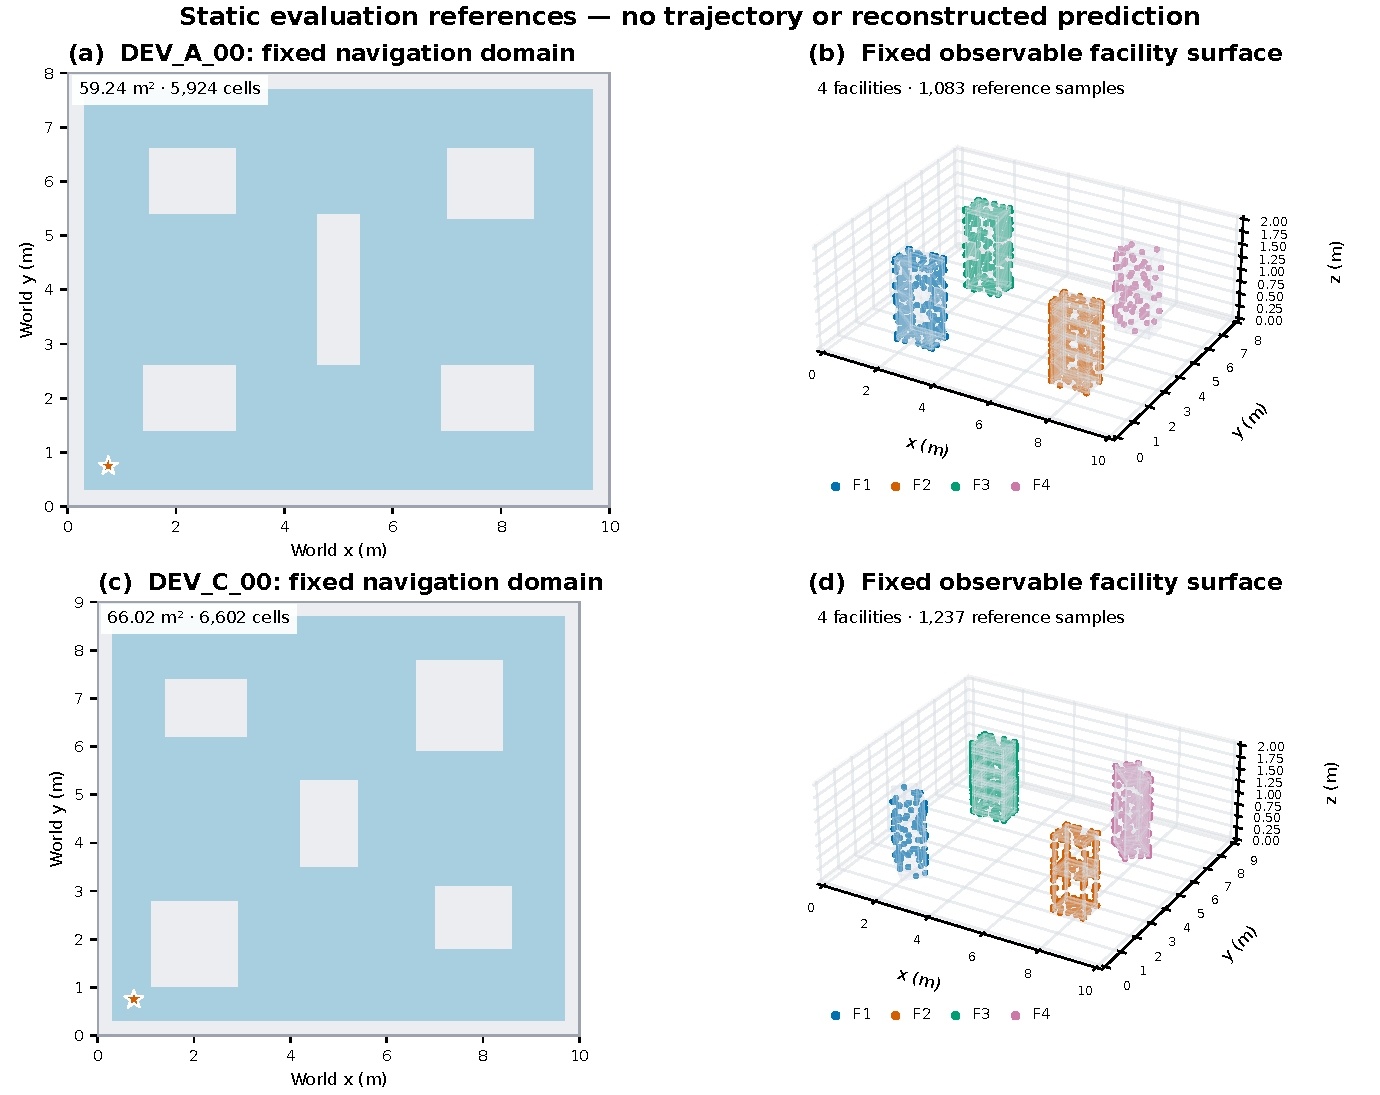
\includegraphics[width=.94\linewidth]{docs/thesis/figures/v44_evaluation_reference/evaluation_reference.pdf}
 \caption{两个开发场景的静态评价参考。左列蓝色格为固定可通行域分母，星形为起点；右列彩色点为可观察设施表面样本，浅灰几何用于定位。F1--F4是设施编号。图中没有机器人轨迹、实测重建或方法性能结果。}
 \label{fig:extension-reference}
\end{figure}

采集先保存传感包与执行记录，再进行一次建图、证据更新和决策。独立进程从保存包重建地图及控制器，逐帧核对证据、完整决策与最终网格，并校验数据和源码摘要；网格允许枚举顺序改变，但不允许删去误差表面。该过程是保存观测的确定性重算，没有再次驱动仿真器，不增加独立任务数，也不能给出未执行策略的反事实终点。不完整记录与未返航任务保留其失败身份。

下一步须分别检验预测值是否变化、动作是否变化、实测质量是否改善，并在几何充分与先验失配条件下保留零增益及负例。接口检查和静态参考只支持实现可核查；只有共同协议下独立执行的G/S任务，才能检验本节控制器的语义增量。
